% !TeX program = xelatex
\documentclass[12pt, a4paper]{ntut-report}
\usepackage{graphicx}
%\usepackage{fontspec}
\usepackage{geometry}
\usepackage{lipsum}
\usepackage{xeCJK}
\usepackage{wallpaper}
\usepackage{pdfpages}
\usepackage{indentfirst}
\usepackage{setspace}
\usepackage{hyperref}
\usepackage{zhnumber}
\usepackage{titlesec}
\usepackage{amsmath,amssymb,amsthm,mathtools,bm}
\usepackage{tabularx}
\usepackage{booktabs,array,longtable}
\usepackage{subcaption}

\captionsetup{justification=centering,singlelinecheck=false,font={normalsize,stretch=2}}
\captionsetup[sub]{justification=centering,singlelinecheck=false,font={normalsize,stretch=2}}

\renewcommand{\baselinestretch}{1.5}
\xeCJKsetup{AutoFakeBold=true, AutoFakeSlant=true}
\setCJKmainfont{AR PL KaitiM Big5} % 中文字體
\setmainfont{Times New Roman} % 英文字體
\geometry{a4paper,total={297mm,210mm},top=4.5cm,bottom=0.75cm,left=2.5cm,right=2.5cm} % 頁面設定，不需修改
\pagestyle{plain} % 頁碼
%
% this file is encoded in utf-8
%

%% 這些設定值將會用於呈現在首頁上，請進行填入
%% Please fill in the information which will be shown on the cover and in the abstract. All Chinese and English information must be matched to each other. If you don’t have any Chinese information, please skip the Chinese ones, but all English Information is required.

%
% 中文論文設定值，請根據以下的範例進行填入
%

% 論文題目（中文）
% Thesis Title (Chinese)
\newcommand\cTitle{階層式聯邦強化學習於 O-RAN IAB 網路之 PRB 資源分配} % TODO: 確認中文題目

% 我的姓名（中文）
% My Name（Chinese）
\newcommand\myCname{（請填入姓名）} % TODO

% 指導教授的姓名 (中文)，使用頓號隔開 
% Advisor (Chinese), use “、” to separate names
\newcommand\advisorCname{（請填入指導教授） 博士} % TODO

% 校名 (中文)
% School Name（Chinese）
\newcommand\univCname{國立臺北科技大學}

% 系所名 (中文)
% Department Name（Chinese）
\newcommand\deptCname{（請填入系所）碩士班} % TODO

% 學位名 (中文)
% Degree Name（Chinese）
\newcommand\degreeCname{碩士}

% 口試年份 (中文、民國)
% Year of Oral Defense（Chinese）
\newcommand\cYear{一百一十五} % TODO: 確認口試年份（民國）

% 口試月份 (中文)
% Month of Oral Defense（Chinese）
\newcommand\cMonth{（月）} % TODO

% 畢業學年度 (中文)
% 如 112 學年度第2學期畢業，當時為民國113年6月，學年度即為112，不是113。
\newcommand\cAcademicYear{（學年度）} % TODO

% 畢業學期（中文）
% Academic Year (Chinese)
\newcommand\cGraduateSemester{（學期）} % TODO

%
% 英文論文設定值，請根據以下的範例進行填入
%

% 論文題目 (英文）
% Thesis Title (Engslih)
\newcommand\eTitle{Hierarchical Federated Reinforcement Learning for PRB Allocation in O-RAN-Controlled Integrated Access and Backhaul Networks} % TODO: confirm title

% 我的姓名（英文）
% My Name（English）
\newcommand\myEname{(Your Name)} % TODO: e.g. Chen, Da-Ming

% 指導教授的姓名 (英文)，使用逗號隔開
% 例如：Dr. Kuo Jong-Yi, Dr. A B-C, ...
%
% Advisor (Ensligh), use “, ” to separate names
% e.g. Dr. Kuo Jong-Yi, Dr. A B-C, ...
\newcommand\advisorEname{Dr. (Advisor Name)} % TODO

% 校名（英文）
% School Name（English）
\newcommand\univEname{National Taipei University of Technology}

% 系所全名 (英文)
% Department Name（English）
\newcommand\fulldeptEname{Department of Electronic Engineering} % TODO

\newcommand\deptEname{Electronic Engineering} % TODO

% 學位名 (英文)
% Degree（English）
\newcommand\degreeEname{Master}

% 口試年份 (阿拉伯數字、西元)
% Year of Oral Defense（English）
\newcommand\eYear{2026} % TODO: confirm

% 口試月份 (英文)
% Month of Oral Defense（English）
\newcommand\eMonth{(Month)} % TODO

%畢業級別；用於書背列印；若無此需要可忽略
\newcommand\GraduationClass{（級別）} % TODO

%%%%%%%%%%%%%%%%%%%%%%

%
% English-thesis settings
% 將模板中的中文標題（第X章、目錄、圖、表、誌謝）改為英文
%
\makeatletter
% Chapter heading: "CHAPTER 1  Introduction"
\renewcommand\prechaptername{CHAPTER~}
\renewcommand\postchaptername{}
\renewcommand\countermapping[1]{\arabic{chapter}}
% Table of contents entry: "Chapter 1  Introduction"
\renewcommand\tocprechaptername{Chapter~}
\renewcommand\tocpostchaptername{}
% Names of lists, captions and references
\renewcommand\contentsname{TABLE OF CONTENTS}
\renewcommand\listfigurename{LIST OF FIGURES}
\renewcommand\listtablename{LIST OF TABLES}
\renewcommand\figurename{Figure}
\renewcommand\tablename{Table}
\renewcommand\tableofcontents{%
    \chapter*{\contentsname}%
    \phantomsection
    \addcontentsline{toc}{chapter}{TABLE OF CONTENTS}%
    \@starttoc{toc}}
\renewcommand\listoffigures{%
    \chapter*{\listfigurename}%
    \phantomsection
    \addcontentsline{toc}{chapter}{LIST OF FIGURES}%
    \@starttoc{lof}}
\renewcommand\listoftables{%
    \chapter*{\listtablename}%
    \phantomsection
    \addcontentsline{toc}{chapter}{LIST OF TABLES}%
    \@starttoc{lot}}
% Acknowledgements page in English
\renewenvironment{Thanks}
{
    \chapter*{ACKNOWLEDGEMENTS}
    \vspace{0.5cm}
    \
    \begin{spacing}{2}
    \phantomsection % for hyperref to register this
    \addcontentsline{toc}{chapter}{ACKNOWLEDGEMENTS}
}
{
    \end{spacing}
    \vspace{0.5cm}
}
% Body chapters (English)
\newenvironment{EnChapter}
{
    \begin{spacing}{2}
}
{
    \end{spacing}
}
\makeatother

%
% Theorem-like environments and notation used in the thesis
%
\newtheorem{definition}{Definition}[chapter]
\newtheorem{assumption}{Assumption}[chapter]
\newtheorem{proposition}{Proposition}[chapter]
\newtheorem{remark}{Remark}[chapter]
\newtheorem{example}{Example}[chapter]

\newcommand{\Nset}{\mathcal{N}}
\newcommand{\Uset}{\mathcal{U}}
\newcommand{\Vset}{\mathcal{V}}
\newcommand{\Eset}{\mathcal{E}}
\newcommand{\Cset}{\mathcal{C}}
\newcommand{\Aset}{\mathcal{A}}
\newcommand{\Tset}{\mathcal{T}}
\newcommand{\Bset}{\mathcal{B}}
\newcommand{\Gset}{\mathcal{G}}
\newcommand{\parent}{p}
\newcommand{\Ind}{\mathbb{1}}
\newcommand{\E}{\mathbb{E}}
\newcommand{\act}{\mathrm{act}}
\DeclareMathOperator{\clip}{clip}
\DeclareMathOperator{\br}{br}
\DeclareMathOperator{\role}{role}

\begin{document}

% 封面、不用浮水印 Cover without a watermark
\begin{titlepage}
    \newpage
    \begin{center}
        % 北科的 Logo（英文版）
        % English NTUT logo; use ntut-logo-with-label.png for the Chinese version
        
\includegraphics[width=13cm]{ntut-logo-with-label-eng.jpg}

        % Department and degree
        \LARGE\bf\fulldeptEname\\% Department (English)
        \LARGE\bf\degreeEname{} Thesis\\% "Master Thesis"

        % English title (Chinese title below it; comment out \cTitle if not needed)
        \vfill
        \LARGE\bf\eTitle\\
        \Large\bf\cTitle\\

        % Researcher
        \vfill
        {\Large Researcher: \myEname}

        % Advisor
        \vfill
        {\Large Advisor: \advisorEname}

        % Date of oral defense
        \vfill
        {\Large \eMonth, \eYear}
    \end{center}
\end{titlepage}

% 留白頁、不用浮水印 Blank page without a watermark
\newpage
\thispagestyle{empty}
% (預留空白頁)

% 新增浮水印 Add Watermarks
\CenterWallPaper{.64}{ntut-logo.png}

% 封面、要浮水印 Cover with a watermark
\begin{titlepage}
    \newpage
    \begin{center}
        % 北科的 Logo（英文版）
        % English NTUT logo; use ntut-logo-with-label.png for the Chinese version
        
\includegraphics[width=13cm]{ntut-logo-with-label-eng.jpg}

        % Department and degree
        \LARGE\bf\fulldeptEname\\% Department (English)
        \LARGE\bf\degreeEname{} Thesis\\% "Master Thesis"

        % English title (Chinese title below it; comment out \cTitle if not needed)
        \vfill
        \LARGE\bf\eTitle\\
        \Large\bf\cTitle\\

        % Researcher
        \vfill
        {\Large Researcher: \myEname}

        % Advisor
        \vfill
        {\Large Advisor: \advisorEname}

        % Date of oral defense
        \vfill
        {\Large \eMonth, \eYear}
    \end{center}
\end{titlepage}

% 「學位論文口試委員會審定書」掃描檔，請檢附完整簽名之審定書掃描檔
% Please add "Oral Defense Committee Signature Form" with complete signatures.
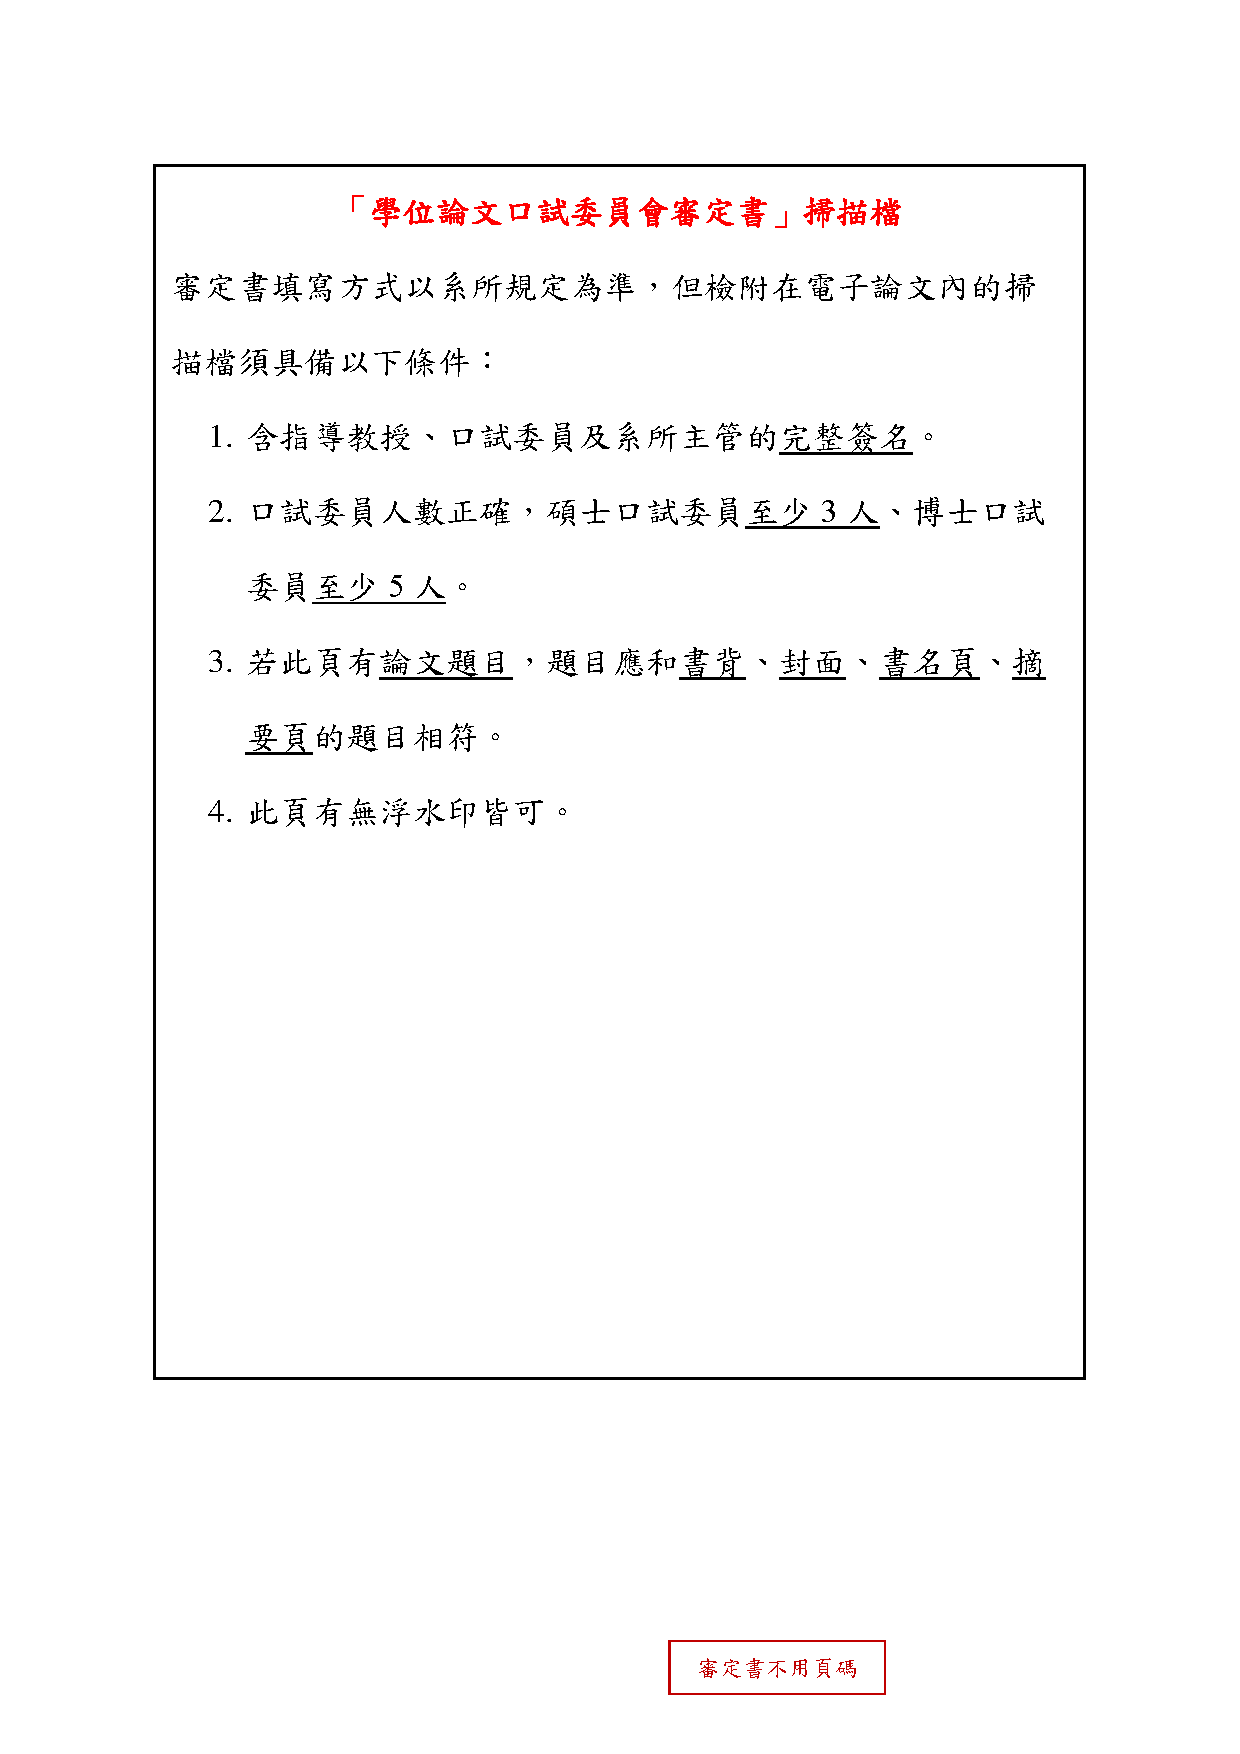
\includepdf[pages=-]{static-page/signpage.pdf}

\pagenumbering{roman}

% 摘要頁（中文）Abstract (Chinese)
% If you don’t have Chinese abstract, please delete this one.
% 中文摘要頁
% TODO: 本摘要為依據系統模型章節撰寫之草稿，待實驗章節完成後補上主要結果。
\begin{ZhAbstract}
    \begin{ZhAbstractItems}
        \noindent 論文名稱：\cTitle

        \noindent 校院系：\univCname\ \deptCname \hfill 頁數：（請填）

        \noindent 畢業時間：\cAcademicYear 學年度第\cGraduateSemester 學期 \hfill 學位：\degreeCname

        \noindent 研究生：\myCname \hfill 指導教授：\advisorCname

        % 關鍵詞，多個關鍵字以頓號(、)隔開
        \noindent 關鍵詞：O-RAN、整合接取與回程（IAB）、PRB 資源分配、多智能體強化學習、階層式聯邦學習

    \end{ZhAbstractItems}

    \begin{ZhAbstractDescription}
        整合接取與回程（IAB）透過多跳無線回程延伸網路覆蓋，然而每個 IAB 節點中的行動終端（MT）與分散單元（DU）必須共享無線資源，且任一跳的壅塞會向下影響整個子樹。本論文研究 O-RAN 控制下 IAB 網路之下行實體資源區塊（PRB）分配問題。本文首先建立與拓撲無關的系統模型，將任意深度的多跳 IAB 網路表示為有根樹，並描述鏈路速率、以回程感知 PRB 預算刻劃的 MT--DU 資源耦合，以及多跳佇列動態，進而定義總吞吐量最大化問題。由於該問題之動作空間呈指數成長、跨時間與跨跳耦合，且通道與需求統計未知，本文將每個 IAB 節點視為一個智能體，於比例公平排程器上施加各子節點之 PRB 上限，並以逐因子近端策略最佳化目標及具排列等變性之策略與價值網路進行訓練。智能體間透過聯邦學習共享知識，由平面 FedAvg 逐步發展為結合 Hedge 權重與發散回退機制之拓撲階層式聚合，最終提出依節點角色個人化廣播模型之 HiRA-Fed。整體架構以 xApp 及輔助服務部署於包含十二個 IAB 節點與十六個使用者設備之 O-RAN 實驗平台。（實驗結果待補。）
    \end{ZhAbstractDescription}

\end{ZhAbstract}

% 摘要頁（英文）Abstract (English)
% 英文摘要頁
% TODO: This is a draft based on the System Model chapter. Add the main
% experimental findings once Chapter 4 is complete.
\begin{EnAbstract}
    \begin{EnAbstractItems}
        \noindent Researcher: \myEname \hfill Advisor: \advisorEname

        \noindent \deptEname, \univEname

        % 關鍵詞，多個關鍵字以逗號 "," 隔開
        \noindent Keywords: O-RAN, integrated access and backhaul (IAB), PRB allocation, multi-agent reinforcement learning, hierarchical federated learning

    \end{EnAbstractItems}

    \begin{EnAbstractDescription}
        Integrated access and backhaul (IAB) extends radio coverage by letting base stations relay traffic wirelessly over multiple hops, but the mobile termination (MT) and the distributed unit (DU) of each IAB node compete for the same radio resources, and congestion at one hop propagates to the whole subtree below it. This thesis studies downlink physical resource block (PRB) allocation in an O-RAN-controlled IAB network. A topology-agnostic system model is developed that represents a multi-hop IAB network of arbitrary depth as a rooted tree and captures the link rates, the MT--DU resource coupling through a backhaul-aware PRB budget, and multi-hop queue dynamics, from which a sum-throughput maximization problem is formulated. Because this problem has an exponentially large and temporally coupled action space and unknown channel and demand statistics, each IAB node is modelled as an agent that imposes per-child PRB caps on a proportional-fair scheduler and is trained with a factor-wise proximal policy optimization objective using permutation-equivariant policy and value networks. Knowledge is shared among agents through federated learning, progressing from flat FedAvg to a topology-hierarchical aggregation with Hedge weighting and divergence fallback, and finally to HiRA-Fed, which personalizes the broadcast model according to the role of each node. The complete framework is deployed as xApps and supporting services on an O-RAN testbed with twelve IAB nodes and sixteen user equipments. (Experimental results to be added.)
    \end{EnAbstractDescription}

\end{EnAbstract}

% 鳴謝 Acknowledgements
\begin{Thanks}
    % TODO: Write your acknowledgements here.
    I would like to express my sincere gratitude to my advisor, \advisorEname, for the guidance and support throughout this research. (To be completed.)
\end{Thanks}

% 目錄、表目錄與圖目錄 Table of Contents, List of tables, List of figures
\begin{TableOfContent}
    \tableofcontents
\end{TableOfContent}

\begin{TableOfContent}
    \listoffigures
\end{TableOfContent}

\begin{TableOfContent}
    \listoftables
\end{TableOfContent}

\pagenumbering{arabic}

% Chapter 1
\begin{EnChapter}

\chapter{Introduction}
\label{chap:introduction}

% TODO: This chapter is a skeleton. Replace the placeholders with your own text.

\section{Background}
\label{sec:background}

(To be written: 5G/6G densification, integrated access and backhaul (IAB), and the
O-RAN architecture with its RAN Intelligent Controllers.)

\section{Motivation}
\label{sec:motivation}

(To be written: why PRB allocation over multi-hop IAB backhaul is difficult ---
MT--DU resource coupling, congestion propagating along the tree, and the limitations
of a proportional-fair scheduler that is unaware of the topology.)

\section{Contributions}
\label{sec:contributions}

(To be written: the main contributions of this thesis, for example the
topology-agnostic system model, the MARL formulation with per-child PRB caps, the
hierarchical federated learning schemes up to HiRA-Fed, and the O-RAN testbed
implementation.)

\section{Thesis Organization}
\label{sec:organization}

The remainder of this thesis is organized as follows.
Chapter~\ref{chap:related-work} reviews related work.
Chapter~\ref{chap:system-model} presents the system model, the optimization problem,
the multi-agent reinforcement learning formulation, the hierarchical federated
learning schemes, and their mapping to the O-RAN architecture.
Chapter~\ref{chap:experiments} describes the experimental setup and results.
Finally, Chapter~\ref{chap:conclusion} concludes the thesis and discusses future work.

\end{EnChapter}

% Chapter 2
\begin{EnChapter}

\chapter{Related Work}
\label{chap:related-work}

% TODO: This chapter is a skeleton. Replace the placeholders with your own text.

\section{Resource Allocation in IAB Networks}

(To be written.)

\section{Reinforcement Learning for RAN Control in O-RAN}

(To be written.)

\section{Federated Learning for Wireless Networks}

(To be written.)

\end{EnChapter}

% Chapter 3
\begin{EnChapter}

\chapter{System Model}
\label{chap:system-model}

This chapter models downlink resource control in a multi-hop integrated access
and backhaul (IAB) network. The model permits arbitrary finite tree depth, unequal
branch depths, and different numbers of IAB nodes and user equipments (UEs).
Each IAB distributed unit (DU) retains its slot-level proportional fair (PF)
scheduler. A local deep reinforcement learning (DRL) agent adjusts the scheduling
eligibility of its directly attached UEs through a joint time-domain mask action;
the mobile terminations (MTs) of downstream IAB nodes remain eligible. Local
learning uses a deep Q-network (DQN) with a subtree-throughput reward. The
federated configuration shares model parameters through sample-weighted federated
averaging (FedAvg). Only PF, pure Local DRL, and Local DRL with FedAvg are defined
here. Numerical testbed settings are separated from the general formulation.

\section{Network Topology}
\label{subsec:topology}

Let $\Nset=\{n_1,\ldots,n_N\}$ be the IAB nodes and
$\Uset=\{u_1,\ldots,u_U\}$ the terminal UEs. The donor is denoted by $0$, and
these three sets of identities are disjoint. Define
\begin{equation}
  \mathbb{T}=(\Vset,\Eset),\qquad
  \Vset=\{0\}\cup\Nset\cup\Uset,\qquad
  \Eset=\{(\parent(v),v):v\in\Nset\cup\Uset\},
\end{equation}
where $\parent(v)\in\{0\}\cup\Nset$ is the unique serving parent of $v$.
The graph is a rooted directed tree with donor $0$ as its root and UEs as leaves.
Thus every UE has a unique downlink route. Multi-parent routing and topology
reconfiguration during a measurement run are outside the present model.

\begin{definition}[Children, depth, and descendants]
For $n\in\{0\}\cup\Nset$, define
\begin{align}
  \Cset_n^{\mathrm{I}}&=\{m\in\Nset:\parent(m)=n\}, &
  \Cset_n^{\mathrm{U}}&=\{u\in\Uset:\parent(u)=n\},\\
  \Cset_n&=\Cset_n^{\mathrm{I}}\cup\Cset_n^{\mathrm{U}}, &
  h(v)&=h(\parent(v))+1,\quad h(0)=0.
\end{align}
The maximum UE hop count is $H=\max_{u\in\Uset}h(u)$. Let $\Uset_v$ be the
terminal UEs descended from vertex $v$, including $v$ when $v$ is itself a UE.
Then
\begin{equation}
  \Uset_u=\{u\},\qquad
  \Uset_n=\Cset_n^{\mathrm{U}}\cup
           \bigcup_{m\in\Cset_n^{\mathrm{I}}}\Uset_m.
  \label{eq:subtree-ues}
\end{equation}
The union in~\eqref{eq:subtree-ues} is disjoint. The ordered downlink path
$\mathcal{P}(u)$ is the sequence of edges from $0$ to $u$.
\end{definition}

Any IAB node may serve both terminal UEs and downstream IAB nodes. A node with
$\Cset_n^{\mathrm{I}}\ne\emptyset$ is called a relay; an IAB node without IAB
children is called an access node. These roles depend on connectivity rather than
on a fixed depth or node identifier. There is no fixed bound on $N$, $U$, $H$, or
$|\Cset_n|$ in the mathematical model.

\paragraph{MT--DU architecture and forwarding.}
Node $n\in\Nset$ contains MT$_n$, attached to DU$_{\parent(n)}$, and DU$_n$,
serving $\Cset_n$. An IAB child appears to its parent's scheduler as one MT
scheduling entity, although that entity carries traffic for every UE in its
subtree. The donor connects to the core network through a wired interface.
The implementation forwards traffic using Linux IP routing over MT PDU sessions;
it does not implement a Backhaul Adaptation Protocol layer. Each child has one
configured data bearer, and the parent observes an aggregated RLC queue towards
that child. The per-flow queues below are an analytical decomposition of these
aggregates, rather than separately exposed queues at the controller.

\begin{example}[Current experimental instance]
The deployed topology has $N=12$, $U=24$, and $H=3$. The donor serves relays
$n_1,\ldots,n_4$. For $i=1,\ldots,4$,
\begin{equation}
  \Cset_{n_i}^{\mathrm{I}}=\{n_{2i+3},n_{2i+4}\},\qquad
  \Cset_{n_i}^{\mathrm{U}}=\{u_{2i+15},u_{2i+16}\}.
\end{equation}
For $i=5,\ldots,12$,
\begin{equation}
  \Cset_{n_i}^{\mathrm{I}}=\emptyset,\qquad
  \Cset_{n_i}^{\mathrm{U}}=\{u_{2i-9},u_{2i-8}\}.
\end{equation}
UEs $u_1,\ldots,u_{16}$ are three hops from the donor; relay-attached UEs
$u_{17},\ldots,u_{24}$ are two hops away. These counts instantiate the model and
are not constants in its queue, reward, or aggregation equations.
\end{example}

\section{Time Structure and Radio Resources}
\label{subsec:resource}

A radio slot is indexed by $t\in\mathbb{Z}_{\ge0}$ and has duration
$T_{\mathrm{slot}}=10^{-3}2^{-\mu}$ seconds, where $\mu$ is the numerology.
All times and rates in this chapter use simulated time unless explicitly stated
otherwise. DU$_n$ has $B_n$ PRBs. Let $\tilde B_n(t)\le B_n$ be the available
PRBs in slot $t$, with $\tilde B_n(t)=0$ when no downlink data can be scheduled.
The set $\Tset_n^{\mathrm{DL}}$ includes downlink-capable slots, including usable
special slots of the configured TDD pattern.

An observation is collected every $\Delta_o$ seconds. A normal decision interval
contains $L_h$ observations, with duration $\Delta_d=L_h\Delta_o$. Decision $k$
begins at slot $t_k$ and is held over $\Tset_k=\{t_k,\ldots,t_{k+1}-1\}$.
A change in the attached-child set may end the hold early and trigger a new
valid action. Node decisions need not be perfectly synchronized; timestamped
observations are aligned during training.

\begin{assumption}[Inter-link radio independence]
\label{ass:orthogonal}
The model assumes out-of-band-like operation: a node's MT reception does not
exclude simultaneous DU transmission, and different DU radio links have no
modelled co-channel interference. On the OAI RF-simulation platform the links use
independent connections with no cross-link interference, even though their
nominal carrier configurations can coincide. This behaviour is not evidence that
all deployed cells use physically non-overlapping carriers. No in-band MT--DU
half-duplex constraint is imposed in this study.
\end{assumption}

The earlier MT-activity-based DU PRB budget reduction is disabled. Consequently,
in a downlink-capable slot the current resource configuration has
\begin{equation}
  \tilde B_n(t)=\lfloor\beta_n(t)B_n\rfloor,\qquad
  \beta_n(t)=1,
  \label{eq:beta}
\end{equation}
subject to the scheduler's ordinary control, reference-signal, and allocation
constraints. Resource competition still exists among the children served by the
\emph{same} DU, and across hops through their traffic and queues.

\section{Link Service and PF Scheduling}
\label{subsec:rate}
\label{subsec:coupling}

Let $q_{n,v}(t)$ be the MCS selected for child $v\in\Cset_n$.
An approximate payload capacity in bits per PRB is
\begin{equation}
  \rho_{n,v}(t)=\nu_{n,v}(t)N_{\mathrm{RE},n,v}^{\mathrm{data}}(t)
               Q_m\bigl(q_{n,v}(t)\bigr)R\bigl(q_{n,v}(t)\bigr),
  \label{eq:rho}
\end{equation}
where $\nu$ is the layer count, $N_{\mathrm{RE}}^{\mathrm{data}}$ is the number of
payload resource elements per PRB, $Q_m$ is the modulation order, and $R$ is the
coding rate. Actual transport-block sizing is performed by OAI; this expression
is a service abstraction, not an application-throughput prediction. Let
$\eta_{n,v}(t)\in[0,1]$ represent the effective successfully delivered payload
fraction, including the effects of retransmissions and protocol overhead.

Let $b_{n,v}(t)$ be the total allocated PRBs, including new transmissions and
HARQ retransmissions. Let $b_{n,v}^{\mathrm{new}}(t)\le b_{n,v}(t)$ be the
new-transmission allocation and $z_{n,v}(t)=\Ind[b_{n,v}^{\mathrm{new}}(t)>0]$.
Ordinary DU constraints include
\begin{equation}
  b_{n,v}(t)\in\mathbb{Z}_{\ge0},\qquad
  \sum_{v\in\Cset_n}b_{n,v}(t)\le\tilde B_n(t),\qquad
  z_{n,v}(t)\le e_{n,v}(t),
  \label{eq:du-budget}
\end{equation}
where $e_{n,v}(t)$ is the new-transmission eligibility indicator, accounting for
attachment, HARQ processes, feedback opportunities, and other MAC constraints.
For example, a finite feedback opportunity $g$ can constrain scheduled
transmissions through
\begin{equation}
  \sum_{t\in\mathcal{F}_{n,v,g}}z_{n,v}(t)\le A_{n,v,g},
  \label{eq:feedback}
\end{equation}
where $\mathcal{F}_{n,v,g}$ contains slots mapped to that opportunity and
$A_{n,v,g}$ is its feedback capacity. This is an abstraction of the configured
feedback mechanism, not a universal fixed transmission limit for all base stations.
Unused PRBs can remain when no other child is eligible; PRB availability alone
therefore does not guarantee that another child can receive them.

PF orders eligible children using their estimated instantaneous supportable rate
relative to their smoothed served rate, abstractly
\begin{equation}
  M_{n,v}(t)=\frac{\widehat R_{n,v}^{\mathrm{inst}}(t)}
                    {\overline R_{n,v}(t)+\epsilon_{\mathrm{PF}}}.
  \label{eq:pf-metric}
\end{equation}
Retransmission allocations follow the existing HARQ rules and consume the same
DU budget. The existing OAI scheduler performs the resulting PRB allocations. DRL does not
replace this scheduler, choose MCS values, or directly assign individual PRBs.

\section{Joint Time-Domain Control}
\label{subsec:action}

Let $\mathcal{M}$ be a finite set of binary masks of width $W$, containing the
all-open mask $m_{\mathrm{PF}}$. Let $\Cset_n^{\mathrm{att}}(k)$ be the children
reported as attached at decision time, including attached children with empty
queues. The eligible mask targets are
\begin{equation}
  \mathcal{D}_n(k)=\Cset_n^{\mathrm{att}}(k)\cap\Cset_n^{\mathrm{U}}.
\end{equation}
The node chooses a \emph{joint} action: a subset of direct UEs and one common mask
for that subset. The candidate set is
\begin{equation}
  \Aset_n(o_n(k))=\{a_{\mathrm{PF}}\}\cup
  \bigl\{(\mathcal{S},m):\emptyset\ne\mathcal{S}\subseteq\mathcal{D}_n(k),
                         m\in\mathcal{M}\setminus\{m_{\mathrm{PF}}\}\bigr\},
  \label{eq:action-set}
\end{equation}
with cardinality
\begin{equation}
  |\Aset_n|=1+(2^{|\mathcal{D}_n|}-1)(|\mathcal{M}|-1).
  \label{eq:action-count}
\end{equation}
The PF action is represented once, independently of subset membership.
For $a_n(k)=(\mathcal{S}_n(k),m_n(k))$, define
\begin{equation}
  m_{n,v}(k)=
  \begin{cases}
    m_n(k),&v\in\mathcal{S}_n(k),\\
    m_{\mathrm{PF}},&v\notin\mathcal{S}_n(k).
  \end{cases}
  \label{eq:child-mask}
\end{equation}
For $a_{\mathrm{PF}}$, every child receives $m_{\mathrm{PF}}$.
In particular, $m_{n,m}=m_{\mathrm{PF}}$ for all IAB children
$m\in\Cset_n^{\mathrm{I}}$: the current policy never masks a downstream MT.

Let $\iota_n(t)\in\{0,\ldots,W-1\}$ be the mask-bit index used by the MAC.
The additional scheduling constraint is
\begin{equation}
  z_{n,v}(t)\le m_{n,v}(k)[\iota_n(t)],\qquad t\in\Tset_k,
  \label{eq:mask-constraint}
\end{equation}
where a one bit permits scheduling and a zero bit excludes new scheduling through
the controlled PF path. The implementation checks the mask in the new-transmission
scheduling path; HARQ retransmissions retain their own scheduling rules. Thus the
constraint models the controlled transmissions, rather than an assurance that no
radio transmission of any kind occurs in a masked slot.

The PRB cap is left at $B_n$ for every child, so PF determines frequency-domain
allocation within eligible slots. The donor also remains unmodified PF.
The mask is an eligibility restriction, not an exclusive slot reservation for
any other child. Its effective allowed downlink fraction is
\begin{equation}
  d_{n,v}(k)=
  \frac{\sum_{t\in\Tset_k}\Ind[t\in\Tset_n^{\mathrm{DL}}]
                          m_{n,v}(k)[\iota_n(t)]}
       {\max\{1,\sum_{t\in\Tset_k}\Ind[t\in\Tset_n^{\mathrm{DL}}]\}}.
  \label{eq:effective-mask}
\end{equation}
Masks with equal bit counts can have different effects because the TDD pattern,
special-slot symbol budgets, and feedback timing also matter. No universal
throughput gain is assumed for time-domain control relative to frequency control.

\section{Multi-Hop Traffic and Queues}
\label{subsec:traffic}

UE $u$ has an offered downlink rate $\lambda_u(k)\ge0$, in bits per simulated
second. Let $A_u(t)$ be new payload bits admitted at the donor. TCP injection is
adapted by transport congestion control; UDP can continue injecting its target
rate even when queues overflow. The offered rate is not an observation supplied
by the scenario to the DRL policy.

For every DU $n$ on $\mathcal{P}(u)$, let $Q_n^{(u)}(t)$ be the buffered bits of
flow $u$, and let $S_n^{(u)}(t)$ be successfully forwarded bits. For child $v$,
\begin{equation}
  Q_{n,v}(t)=\sum_{u\in\Uset_v}Q_n^{(u)}(t),\qquad
  S_{n,v}(t)=\sum_{u\in\Uset_v}S_n^{(u)}(t).
\end{equation}
An abstract aggregate service limit is
\begin{equation}
  0\le S_{n,v}(t)\le
  \min\{Q_{n,v}(t),\eta_{n,v}(t)b_{n,v}(t)\rho_{n,v}(t)\}.
  \label{eq:queue-agg}
\end{equation}
Per-hop arrival conservation is
\begin{equation}
  A_0^{(u)}(t)=A_u(t),\qquad
  A_n^{(u)}(t)=S_{\parent(n)}^{(u)}(t-\tau_n),\quad n\in\Nset,
  \label{eq:flow-conservation}
\end{equation}
where $\tau_n\ge1$ is an abstract forwarding delay in slots and service before
slot zero is zero. Arrivals are placed in the queue after the current-slot
service. With capacity $Q_{n,v}^{\max}$ and
$A_{n,v}=\sum_{u\in\Uset_v}A_n^{(u)}$, queue evolution and overflow are
\begin{align}
  Q_{n,v}(t+1)&=\min\{Q_{n,v}^{\max},\ Q_{n,v}(t)-S_{n,v}(t)+A_{n,v}(t)\},
  \label{eq:queue}\\
  D_{n,v}(t)&=[Q_{n,v}(t)-S_{n,v}(t)+A_{n,v}(t)-Q_{n,v}^{\max}]^+.
  \label{eq:drop}
\end{align}
These equations apply at every depth. Aggregate service is split among flows in
queue order; flow-level queues are bookkeeping variables for end-to-end accounting.
Finite buffers keep occupancies bounded, but bounded queues alone do not imply
that every offered flow is fully supported.

The radio-delivered terminal rate and its long-term constraints are
\begin{align}
  x_u^{\mathrm{rad}}(k)&=\frac{1}{\Delta_k}
                  \sum_{t\in\Tset_k}S_{\parent(u),u}(t),
                  \qquad \Delta_k=|\Tset_k|T_{\mathrm{slot}},
  \label{eq:ue-tput}\\
  \overline x_u^{\mathrm{rad}}&\le\overline\lambda_u, &
  \sum_{u\in\Uset_v}\overline x_u^{\mathrm{rad}}
      &\le\limsup_{T\to\infty}\frac{1}{TT_{\mathrm{slot}}}
                \sum_{t=0}^{T-1}\E[S_{\parent(v),v}(t)].
  \label{eq:link-cap}
\end{align}
These are necessary flow constraints, not a sufficient characterization of all
feasible allocations under HARQ, PF, and transport dynamics. Backhaul bytes are
intermediate traffic and must not be added again to terminal throughput.

\section{Optimization Objective and Evaluation}
\label{subsec:problem}

Let $x_u^{\mathrm{app}}(k)$ be the unique payload delivered to the UE application
per simulated second over interval $k$. It can differ from the radio rate because
of overhead, retransmissions, reordering, and measurement boundaries. The target
of the control policy is end-to-end sum goodput,
\begin{equation}
  \textbf{(P1)}\quad
  \max_{\pi}\ \frac{1}{\sum_{k=0}^{K-1}\Delta_k}
     \sum_{k=0}^{K-1}\Delta_k\,
         \E_\pi\!\left[\sum_{u\in\Uset}x_u^{\mathrm{app}}(k)\right],
  \label{eq:P1}
\end{equation}
subject to~\eqref{eq:du-budget},~\eqref{eq:action-set},
\eqref{eq:mask-constraint}, and~\eqref{eq:queue-agg}--\eqref{eq:drop}.
The donor uses $a_{\mathrm{PF}}$; the learned policy comprises only agents
$n\in\Nset$. For equal interval lengths this is the ordinary average sum goodput.
For congestion-only evaluation, the intervals in (P1) are restricted to the
predefined congestion measurement windows, with identical warm-up exclusions
for all methods. Scenario labels select evaluation windows and diagnostic
categories; they are not policy inputs.

Demand satisfaction and its fairness can be reported separately. For
$\Uset^+(k)=\{u:\lambda_u(k)>0\}$, define
\begin{equation}
  \sigma_u(k)=\min\{1,x_u^{\mathrm{app}}(k)/\lambda_u(k)\},\qquad
  J(k)=\frac{\bigl(\sum_{u\in\Uset^+(k)}\sigma_u(k)\bigr)^2}
             {|\Uset^+(k)|\sum_{u\in\Uset^+(k)}\sigma_u(k)^2}.
  \label{eq:satisfaction}
\end{equation}
$J(k)$ is undefined if there are no positive-demand UEs or all satisfaction ratios
are zero; such windows are identified rather than silently treated as perfect
fairness. The current Local DRL and FedAvg comparison optimizes throughput;
there is no implemented satisfaction constraint or Lagrangian fairness update
in this formulation.

Joint actions interact through downstream arrivals and transport feedback.
A higher served backhaul rate helps the objective only if the downstream path
ultimately delivers additional terminal payload. Restricting low-efficiency
direct UEs can increase subtree throughput when the downstream gain exceeds the
direct-UE loss; it can reduce throughput when downstream demand is already met.
Neither this gain nor a benefit from combining relay and access controls is
guaranteed by queue occupancy alone.

\section{Local DQN Formulation}
\label{subsec:marl}

\paragraph{Decentralized interaction.}
Each $n\in\Nset$ is an independently learning agent in a partially observable
multi-agent environment. The global state contains channels, queues, transport
state, and scheduler eligibility. The agent receives $o_n(k)$, selects
$a_n(k)\in\Aset_n(o_n(k))$, and later receives a subtree reward. Other agents'
policies can change during training, so the local environment is non-stationary.
Independent DQN and federated parameter sharing are approximations; they do not
provide a proof of optimality or convergence for (P1).

\paragraph{Observation.}
For a child $v$ reported as attached, let $Y_{n,v}^{\mathrm{prev}}(k)$ be the MAC downlink
transport-block bytes in the observation interval immediately preceding decision
$k$, $\widetilde Q_{n,v}(k)=Q_{n,v}(t_k)/8$ the reported queue in bytes, and
$q_{n,v}(k)$ the latest reported MCS. With reference values $Y_{\mathrm{ref}}$,
$Q_{\mathrm{ref}}$, and $q_{\mathrm{ref}}$, define
\begin{equation}
  \bm z_{n,v}(k)=\left[
  \frac{\log(1+Y_{n,v}^{\mathrm{prev}}(k))}{\log(1+Y_{\mathrm{ref}})},
  \frac{q_{n,v}(k)}{q_{\mathrm{ref}}},
  \frac{\log(1+\widetilde Q_{n,v}(k))}{\log(1+Q_{\mathrm{ref}})},
  \Ind[v\in\Cset_n^{\mathrm{I}}],
  \Ind[m_{n,v}(k-1)\ne m_{\mathrm{PF}}]\right].
  \label{eq:child-feature}
\end{equation}
The stored field named \texttt{wb\_cqi} carries MCS in this implementation, not
an independently measured CQI. Normalization references set the scale; log-scaled
features can exceed one if measurements exceed their references.

Let $L_j^{\mathrm{buf}}(k)$ be the sum of the latest RLC queue bytes reported by
DU$_j$. Neighbour observations give
\begin{align}
  \hat p_n(k)&=\clip\!\left(
       \frac{\log(1+L_{\parent(n)}^{\mathrm{buf}}(k))}
            {\log(1+Q_{p,\mathrm{ref}})},0,1\right),
  \label{eq:phat}\\
  \hat c_n(k)&=\clip\!\left(
       \frac{\log(1+\sum_{m\in\Cset_n^{\mathrm{I}}}L_m^{\mathrm{buf}}(k))}
            {\log(1+\max\{1,|\Cset_n^{\mathrm{I}}|\}Q_{\mathrm{ref}})},0,1\right).
  \label{eq:chat}
\end{align}
Only fresh available measurements enter these expressions. A missing or stale
parent measurement yields $\hat p_n=0$; no fresh IAB-child measurements yields
$\hat c_n=0$. Partial child information uses only the fresh children in the
numerator. $\hat p_n$ describes total parent congestion, not the specific parent
queue serving MT$_n$, so upstream congestion of another branch can also raise it.
For nodes directly below the donor, it is zero in the current implementation,
which does not collect donor relational data.

The complete observation is
\begin{equation}
  o_n(k)=\left(\{\bm z_{n,v}(k)\}_{v\in\Cset_n^{\mathrm{att}}(k)},\ \bm g_n(k)\right),
  \qquad
  \bm g_n(k)=\left[\frac{|\Cset_n^{\mathrm{att}}(k)|}{C_{\max}},
                  \widetilde\phi_n(k),\ \beta_n(k),\ \hat p_n(k),\ \hat c_n(k)\right].
  \label{eq:observation}
\end{equation}
The context $\widetilde\phi_n$ is the retained normalized Global xApp fairness
signal. When enabled, the signal compares recent mean node throughput with that
of nodes having the same topological role:
\begin{equation}
  \widetilde\phi_n=
  \frac{\clip(\overline T_{\mathrm{role}(n)}/(\overline T_n+\epsilon),0.5,2)-0.5}{1.5}.
  \label{eq:fairness-feature}
\end{equation}
When no signal is available, or the feature is disabled, its neutral value is
$1/3$. This is a soft observation feature, not a PRB budget or an FL weight.
Its enabled/neutral setting is identical in the Local-only and FedAvg experiments.
There is no proposed global bottleneck broadcast implemented by the equations here.

\paragraph{Subtree reward and measurement distinction.}
Let $\widehat x_u(\ell)$ be the terminal UE MAC throughput proxy in observation
interval $\ell$. Write $Y_{n,v}(\ell)$ for the MAC byte count collected
during that interval. The proxy is converted to Mbps per simulated second:
\begin{equation}
  \widehat x_u(\ell)=\frac{8\,Y_{\parent(u),u}(\ell)}{10^6\Delta_o}.
  \label{eq:mac-proxy}
\end{equation}
The general subtree utility and current reward are
\begin{align}
  r_n^{(\alpha)}(\ell)&=\sum_{u\in\Uset_n}U_\alpha(\widehat x_u(\ell)), &
  U_\alpha(x)&=
  \begin{cases}
    x^{1-\alpha}/(1-\alpha),&\alpha\ne1,\\
    \log(x+\epsilon_x),&\alpha=1,
  \end{cases}\\
  r_n(\ell)&=r_n^{(0)}(\ell)=\sum_{u\in\Uset_n}\widehat x_u(\ell).
  \label{eq:reward}
\end{align}
No MT throughput is added to this sum, preventing within-reward double counting
of forwarded terminal traffic. For arbitrary tree depth, the terminal set is
computed recursively by~\eqref{eq:subtree-ues}. In the current two-IAB-tier
implementation, a relay reward joins its own terminal-UE measurements with those
of its two access children. Timestamp joins outside the allowed tolerance are
discarded. Missing descendant measurements are not interpreted as zero reward.
Extending the implementation to deeper trees requires discovering all descendant
terminal-serving nodes and aligning their measurements.

The training reward is a MAC-derived proxy, whereas (P1) is assessed using
receiver-side application delivery. Also, rewards of ancestor and descendant
agents overlap: $\sum_{n\in\Nset}r_n$ is generally not the network sum throughput.
The use of subtree rewards encourages consideration of downstream delivery, but
neither makes local maximization exactly equivalent to (P1) nor removes
cross-branch effects.

\paragraph{Action holds and multi-step returns.}
The observation-level rewards belonging to one held decision are averaged:
\begin{equation}
  \overline r_n(k)=\frac{1}{L_{n,k}}
            \sum_{\ell\in\mathcal{H}_{n,k}}r_n(\ell),\qquad
            L_{n,k}=|\mathcal{H}_{n,k}|,
  \label{eq:hold-reward}
\end{equation}
where $\mathcal{H}_{n,k}$ contains the observations from that decision.
The merged transition retains the initial observation, the joint action, the
mean reward, and the observation after the hold. An incomplete group lacking
its initial decision record is discarded. Time-contiguous decision transitions
produce
\begin{equation}
  G_{n,k}^{(m)}=\sum_{j=0}^{m-1}\gamma^j\overline r_n(k+j),\qquad 1\le m\le n_{\mathrm{step}}.
  \label{eq:nstep-return}
\end{equation}
A discontinuity truncates the return. The discount $\gamma$ is per decision,
not per radio slot. The current pipeline stores a bootstrap discount $\gamma^m$
for a retained truncated sequence; truncation is not automatically an absorbing
terminal state. Phase-separated offline training and validation must construct
returns within their own partitions. A random split of overlapping online
multi-step transitions is only a training diagnostic, not an independent
performance test.

\paragraph{Q function and action selection.}
The online network $Q_{\theta_n}(o,a)$ estimates the discounted subtree return.
Its target network is $Q_{\theta_n^-}(o,a)$. The joint action is encoded by
per-child subset indicators and a mask-tier one-hot vector. In the current flat
network,
\begin{equation}
  Q_{\theta_n}(o,a)=c_Q f_{\theta_n}
       \bigl([\operatorname{pad}_{C_{\max}}(o),\ \bm g^{\mathrm{apply}}(a),
                   \operatorname{onehot}(m(a))]\bigr),
  \label{eq:q-network}
\end{equation}
where $c_Q>0$ rescales the network output and $\bm g^{\mathrm{apply}}$ is a
binary vector indicating the selected children. The flat MLP has two hidden
layers. It uses the same input layout at every node; it is not invariant to
permutations of child positions. A consistent child-to-position mapping is
therefore necessary, and permutation robustness must be measured rather than
assumed. Shared set or additive networks available as alternative code paths
are not substituted for the current flat network in this formulation.

The greedy candidate is
\begin{equation}
  a_n^*(k)=\operatorname*{arg\,max}_{a\in\Aset_n(o_n(k))}Q_{\theta_n}(o_n(k),a).
\end{equation}
An optional PF margin $\delta\ge0$, in return units, yields
\begin{equation}
  a_n^{\mathrm{greedy}}(k)=
  \begin{cases}
    a_n^*(k),&Q_{\theta_n}(o_n(k),a_n^*)-Q_{\theta_n}(o_n(k),a_{\mathrm{PF}})>\delta,\\
    a_{\mathrm{PF}},&\text{otherwise}.
  \end{cases}
  \label{eq:pf-margin}
\end{equation}
Training uses $\epsilon$-greedy exploration over valid joint actions, with a
configurable exploration distribution; evaluation sets $\epsilon=0$ and freezes
learning. A PF-only warm start is optional, while pretrained models can start
without it. The margin tests a learned return estimate, not a guaranteed goodput
improvement. The PF margin is an inference rule; the Double DQN target below
still maximizes over the full valid candidate set.

\paragraph{Double DQN update.}
For a replay transition with $m$ observed decisions, define
\begin{align}
  a'&=\operatorname*{arg\,max}_{a\in\Aset_n(o')}Q_{\theta_n}(o',a),\\
  y&=G_{n,k}^{(m)}+\gamma^m Q_{\theta_n^-}(o',a'),
  \label{eq:ddqn-target}\\
  \mathcal{L}_n(\theta_n)&=\frac{1}{|\mathcal{B}_n|}
          \sum_{(o,a,G,o',m)\in\mathcal{B}_n}
          \operatorname{Huber}\!\left(\frac{Q_{\theta_n}(o,a)-y}{c_Q}\right),
  \label{eq:dqn-loss}\\
  \theta_n&\leftarrow\operatorname{AdamStep}(\theta_n,\nabla\mathcal{L}_n;\eta_Q), &
  \theta_n^-&\leftarrow(1-\tau)\theta_n^-+\tau\theta_n.
  \label{eq:polyak}
\end{align}
The implemented Huber threshold is one in normalized network-output units;
gradients are clipped before the Adam update. All structurally valid DQN replay
samples may update the Q network; the old PPO contention gate, probability-ratio
clipping, and actor--critic advantage objective do not apply.

\paragraph{Offline-to-online replay.}
Exploration data provide initialization and continue to be mixed with online
experience. For $M_n^{\mathrm{on}}$ online decisions and an offline pool of size
$M_n^{\mathrm{pool}}$, the number sampled from the offline pool is
\begin{equation}
  M_n^{\mathrm{off}}=\min\{M_n^{\mathrm{pool}},
              \max(\lfloor\zeta M_n^{\mathrm{on}}\rfloor,M_{\min}^{\mathrm{off}})\}.
  \label{eq:offline-mix}
\end{equation}
Thus $\zeta$ is an offline-to-online count ratio, not directly the offline
fraction of the combined batch. Action holds and returns are prepared
consistently for both sources. Invalid actions or incompatible state encodings
are excluded. The same preprocessing is used by the Local training service and
FL clients. Learning is off-policy, but adequate coverage of meaningful actions
and demand/channel conditions is still needed to limit unsupported Q estimates.

\section{Sample-Weighted Federated Averaging}
\label{subsec:fl}

\paragraph{Participants and local computation.}
Federated rounds are launched every $\Delta_{\mathrm{FL}}$ simulated seconds.
The federated clients are the IAB-node agents $\Nset$, excluding the donor.
All use the same Q-network architecture, feature meanings, normalization, mask
menu, reward, discount, and replay processing. Let
$\Theta_n=(\theta_n,\theta_n^-)$ include the online and target parameters; the
legacy checkpoint names \texttt{actor} and \texttt{critic} refer to these two
Q networks in DQN mode, not to an actor--critic algorithm.
At round $r$, participating client $n\in\mathcal{P}_r\subseteq\Nset$ receives
$\Theta_{\mathrm{glob}}^{(r-1)}$ and performs $E_{\mathrm{FL}}$ local DQN updates
on its processed dataset $\mathcal{D}_n^{(r)}$:
\begin{equation}
  \Theta_n^{(r)}=\operatorname{LocalDQN}_{E_{\mathrm{FL}}}
                 (\Theta_{\mathrm{glob}}^{(r-1)},\mathcal{D}_n^{(r)}).
\end{equation}
Background Local training also continues between federated rounds. Local
optimizers and training counters are retained; they are not averaged.

\paragraph{Aggregation and broadcast.}
Let $w_n^{(r)}$ be the number of valid training decision samples in the client's
training partition after preprocessing, including any offline samples actually
included there. It is neither an equal-node weight nor a count restricted to
PPO-contended samples, and it is not multiplied by the number of update epochs.
A client that cannot perform a valid training update reports zero weight.
For $W^{(r)}=\sum_{n\in\mathcal{P}_r}w_n^{(r)}>0$, standard FedAvg is
\begin{equation}
  \Theta_{\mathrm{glob}}^{(r)}=
        \sum_{n\in\mathcal{P}_r}\frac{w_n^{(r)}}{W^{(r)}}\Theta_n^{(r)}.
  \label{eq:fedavg}
\end{equation}
Both online and target networks are averaged with these weights. The result is
published to all configured clients, including zero-weight clients, and becomes
available to inference through checkpoint reload. If $W^{(r)}=0$, aggregation is
skipped and no new averaged model is broadcast. Clients retain their current
local state. Aggregation and reload introduce delay; nodes need not hold
identical parameters between rounds because they continue local updates.

FedAvg exchanges parameters and sample counts rather than raw local replay
records through the FL protocol. The experimental services are nevertheless
co-located on PC1 and use shared database infrastructure. This deployment does
not establish physical data isolation, cryptographic privacy, or an additional
privacy guarantee. FedAvg does not directly distribute radio slots or PRBs,
and its potential goodput benefit is an empirical question under heterogeneous
node data.

\paragraph{Controlled comparison.}
Stage 1 is PF, Stage 1.5 is pure Local DQN, and Stage 2 adds FedAvg to that same
Local design. The Local architecture, initialization, offline data, optimizer
initial state, observation features, actions, reward, exploration schedule,
background-update settings, and training-seed schedule are held identical.
Stage 1.5 restarts from the common initial state and does not inherit Stage 2's
online replay or trained models. FedAvg contributes additional client updates
as well as parameter sharing; both the Local and FL update counts must be
reported, and equal-computation controls are needed to isolate sharing from
extra optimization work. Checkpoint selection uses validation data, with final
performance measured on seeds excluded from tuning and with repeated runs.

\section{Mapping to the O-RAN Architecture}
\label{subsec:oran}

The platform contains OAI E2 nodes and a FlexRIC Near-RT RIC. Local xApps collect
MAC statistics, relay observations through ZeroMQ, and enforce the returned
per-child masks using the custom MAC control path. A Python service called
``Local rApp'' supplies DQN inference and background training. The Flower server
and clients form the service called ``Global rApp''. These names denote custom
services in this implementation; no Non-RT RIC, A1 interface, or SMO is deployed,
so these services are not claimed to be standard Non-RT RIC rApps. Global xApp
observation broadcasting and Global rApp federated aggregation are distinct
functions.

\paragraph{Time conversion.}
With simulator speed $S_{\mathrm{sim}}$, elapsed time and measured rates obey
\begin{equation}
  T_{\mathrm{sim}}=S_{\mathrm{sim}}T_{\mathrm{wall}},\qquad
  R_{\mathrm{sim}}=R_{\mathrm{wall}}/S_{\mathrm{sim}}.
  \label{eq:sim-time}
\end{equation}
Software timers are configured in wall-clock units and converted by this rule;
radio slot duration is already a simulated-time quantity and is not multiplied
again. The current setting is $S_{\mathrm{sim}}=0.3$.

\begin{table}[htbp]
\centering
\small
\caption{Current deployment periods, expressed in simulated time.}
\label{tab:oran-mapping}
\begin{tabular}{@{}p{0.31\textwidth}p{0.40\textwidth}p{0.19\textwidth}@{}}
\toprule
Function & Implementation & Period \\
\midrule
Slot-level PF & OAI DU MAC & 0.5 ms \\
MAC indication & Custom E2SM-MAC report & 0.03 s \\
Observation and control refresh & Local xApp / ZeroMQ & 0.3 s \\
Joint-action decision & Local DQN service & 1.5 s \\
Background Local training & Local DQN service & 18 s \\
Global observation broadcast & Global xApp, when enabled & 0.6 s \\
FedAvg round launch & Flower scheduler, Stage 2 & 54 s \\
Checkpoint reload polling & Local DQN service & 9 s \\
\bottomrule
\end{tabular}
\end{table}
These are configured periods, not upper bounds on end-to-end completion latency.
The ZMQ timeout is a wall-clock software deadline; it is not a radio-slot deadline.
If communication fails, the xApp requests PF fallback. A stalled control process
can leave the previous mask stored in the MAC, so actual enforcement and phase
transitions must be checked independently of inference decisions.

\paragraph{Current numerical instance.}
The deployed numerology is $\mu=1$, with $B_n=106$ PRBs and a 10-slot TDD period:
seven full downlink slots, one special slot with six downlink symbols, and two
uplink slots. The mask width is $W=16$. The MAC uses
$\iota_n(t)=s_n(t)\bmod16$, where $s_n(t)$ is the slot index within a radio frame;
it does not use the absolute slot index modulo 16. The finite menu is
\begin{equation}
  \mathcal{M}=\{\mathtt{0x0101},\mathtt{0x1111},\mathtt{0x9044},
                 \mathtt{0x9292},\mathtt{0xab98},\mathtt{0xffff}\}.
\end{equation}
The current formulation uses $L_h=5$, $\gamma=0.5$, $n_{\mathrm{step}}=3$,
$\alpha=0$, $\tau=0.01$, $c_Q=50$, and minibatches of 128 decisions. The flat
Q network has two 128-unit hidden layers. Learning rate, exploration parameters,
PF margin, offline-mixing ratio, and Local/FL update counts are run-specific
settings and must be reported from the executed configuration and checkpoints,
not inferred from source-code defaults. Learning is disabled and exploration is
zero during final evaluation.

\paragraph{Scope of generalization.}
Topology size enters the equations through sets and descendant relationships,
not through fixed node numbers. Nevertheless, the present code uses a padded
capacity $C_{\max}=16$ children per DU and explicit mappings for the experimental
parent/child relationships and reward joins. A larger or deeper deployment
requires configuring those relationships, recursively collecting descendant
terminal measurements, and retaining correct MT/UE identities. If a DU exceeds
$C_{\max}$, the current flat encoding and network dimensions must be expanded
and compatible models prepared; the present implementation must not be treated
as supporting that case unchanged.

For any finite deployment one can choose
$C_{\max}\ge\max_n|\Cset_n|$ and retain a common input layout for FedAvg.
However, enumerating~\eqref{eq:action-count} costs exponentially many candidates
in the number of attached direct UEs, so increasing UE count can require
candidate pruning or another structured action search. Generalized notation does
not prove scalability, permutation robustness, or transferable goodput gains.
Different depths, fan-outs, demand levels, channel conditions, and feedback
configurations require separate evaluation.

\section{Notation}
\label{subsec:notation}

\begin{longtable}{@{}p{0.28\textwidth}p{0.66\textwidth}@{}}
\toprule
Symbol & Meaning \\
\midrule
\endhead
$\Nset,\Uset,\parent(v)$ & IAB-node set, terminal-UE set, serving parent \\
$\Cset_n^{\mathrm{I}},\Cset_n^{\mathrm{U}}$ & IAB children (MT entities), directly attached UEs \\
$h(v),H,\mathcal{P}(u),\Uset_n$ & Depth, maximum UE hop count, downlink path, subtree terminal UEs \\
$\Delta_o,\Delta_d,L_h,\Tset_k$ & Observation interval, normal decision interval, hold length, decision slots \\
$B_n,\tilde B_n,\beta_n$ & Total PRBs, available PRBs, available fraction \\
$b_{n,v},z_{n,v},e_{n,v}$ & Total allocated PRBs, new-transmission indicator, MAC eligibility \\
$\rho_{n,v},\eta_{n,v}$ & Payload capacity per PRB, effective delivery fraction \\
$\mathcal{M},W,\iota_n(t)$ & Mask menu, mask width, MAC mask-bit index \\
$\Aset_n,a_{\mathrm{PF}},\mathcal{S}_n$ & Valid joint actions, all-open action, selected direct UEs \\
$Q_{n,v},A_{n,v},S_{n,v},D_{n,v}$ & Aggregate queue, arrival bits, forwarded bits, dropped bits \\
$\lambda_u,x_u^{\mathrm{app}},\widehat x_u$ & Offered rate, application goodput, MAC throughput proxy \\
$\bm z_{n,v},\bm g_n,\hat p_n,\hat c_n$ & Child features, node context, upstream/downstream congestion proxies \\
$C_{\max},Y_{\mathrm{ref}},Q_{\mathrm{ref}}$ & Padded child capacity, byte-count normalization references \\
$r_n,\overline r_n,G_{n,k}^{(m)}$ & Observation reward, hold-averaged reward, multi-step return \\
$\gamma,n_{\mathrm{step}},\delta,c_Q$ & Per-decision discount, return length, PF margin, Q output scale \\
$\theta_n,\theta_n^-,\tau,\eta_Q$ & Online/target parameters, Polyak factor, learning rate \\
$\zeta,M_n^{\mathrm{off}}$ & Offline-to-online count ratio, sampled offline decisions \\
$\Theta_n,w_n^{(r)},\mathcal{P}_r$ & FL parameter pair, valid training-sample weight, responding clients \\
$\Delta_{\mathrm{FL}},S_{\mathrm{sim}}$ & Federated launch interval, simulator speed factor \\
\bottomrule
\end{longtable}

\end{EnChapter}

% Chapter 4
\begin{EnChapter}

\chapter{Experimental Results}
\label{chap:experiments}

% TODO: This chapter is a skeleton. Replace the placeholders with your own text.

\section{Experimental Setup}

(To be written: testbed hardware and software, traffic scenarios, and the
parameters listed in Section~\ref{subsec:oran}.)

\section{Baselines and Evaluation Metrics}

(To be written: PF baseline (Stage 1), pure Local DQN (Stage 1.5), Local DQN with FedAvg (Stage 2), and the metrics of
Section~\ref{subsec:problem}, such as sum throughput, demand-satisfaction ratio and
Jain's fairness index.)

\section{Results and Discussion}

(To be written.)

\end{EnChapter}

% Chapter 5
\begin{EnChapter}

\chapter{Conclusion and Future Work}
\label{chap:conclusion}

% TODO: This chapter is a skeleton. Replace the placeholders with your own text.

\section{Conclusion}

(To be written.)

\section{Future Work}

(To be written.)

\end{EnChapter}


% 參考文獻，請在段落上隨意註解，你同時需要 reference.bib
% References omitted from the current draft; source files are retained.
% \renewcommand{\bibname}{REFERENCES}
\begin{thebibliography}{99}
\addcontentsline{toc}{chapter}{REFERENCES}

\bibitem{3gpp38340}
3GPP, ``NR; Backhaul Adaptation Protocol (BAP) Specification,''
Technical Specification TS 38.340.

\bibitem{3gpp38214}
3GPP, ``NR; Physical Layer Procedures for Data,''
Technical Specification TS 38.214.

\bibitem{3gpp38306}
3GPP, ``NR; User Equipment (UE) Radio Access Capabilities,''
Technical Specification TS 38.306.

\bibitem{jain1984fairness}
R. Jain, D.-M. Chiu, and W. R. Hawe,
``A Quantitative Measure of Fairness and Discrimination for Resource Allocation
in Shared Computer Systems,'' Digital Equipment Corporation, Research Report
DEC-TR-301, 1984.

\bibitem{schulman2017ppo}
J. Schulman, F. Wolski, P. Dhariwal, A. Radford, and O. Klimov,
``Proximal Policy Optimization Algorithms,'' arXiv:1707.06347, 2017.

\bibitem{mcmahan2017fedavg}
B. McMahan, E. Moore, D. Ramage, S. Hampson, and B. Ag\"uera y Arcas,
``Communication-Efficient Learning of Deep Networks from Decentralized Data,''
in \emph{Proc. 20th Int. Conf. Artificial Intelligence and Statistics},
vol. 54, pp. 1273--1282, 2017.

\bibitem{sattler2021cfl}
F. Sattler, K.-R. M\"uller, and W. Samek,
``Clustered Federated Learning: Model-Agnostic Distributed Multitask
Optimization Under Privacy Constraints,'' \emph{IEEE Trans. Neural Networks
and Learning Systems}, vol. 32, no. 8, pp. 3710--3722, 2021.

\bibitem{freund1997hedge}
Y. Freund and R. E. Schapire,
``A Decision-Theoretic Generalization of On-Line Learning and an Application
to Boosting,'' \emph{Journal of Computer and System Sciences}, vol. 55, no. 1,
pp. 119--139, 1997.

\end{thebibliography}


\end{document}
